\chapter{Measurement Campaign and Ground Truth}\label{ch:3}

Every claim made in this thesis rests on the quality of the measurement underneath it, and this chapter describes how that measurement was obtained. Section 3.1 describes the instrumentation. Section 3.2 describes the four campaigns and the routes they cover. Section 3.3 describes the signalling-decoding procedure and the configuration-timeline correction that it required. Section 3.4 describes how continuous driving is segmented into drives and quality controlled. Section 3.5 reports the deployed mobility configuration recovered from the signalling, and Section 3.6 summarises the resulting dataset.


\section{Instrumentation}
\label{sec:3_1}

Measurements were collected with a commercial drive-test handset running Accuver XCAL, which exposes the chipset diagnostic interface and produces two synchronised outputs: a tabular radio-measurement export sampled at one hertz, and a decoded control-plane log containing the RRC messages exchanged between the handset and the network. The use of this class of instrumentation for RRC extraction on live networks follows established practice in the measurement literature \cite{ref5}, \cite{ref4}.

The radio export carries, per sample, the serving-cell physical cell identity (PCI), E-UTRA absolute radio frequency channel number (EARFCN), RSRP, RSRQ and signal-to-interference-plus-noise ratio (SINR), together with GPS-derived speed and heading. Neighbour-cell radio measurements, which are unpopulated in the raw periodic export, are recovered directly from decoded RRC measurement reports and projected onto the 1 Hz sample grid. The signalling log carries the complete RRCConnectionReconfiguration, MeasurementReport and RRCConnectionReestablishment message sequence with millisecond timestamps.

Using the signalling log rather than a vendor handover counter is a deliberate design choice and is the foundation of the ground truth used throughout. A counter reports that the vendor's internal logic considered a handover to have occurred; a decoded RRCConnectionReconfiguration carrying mobilityControlInfo is the handover command, timestamped at the diagnostic logging instant when the message was decoded at the baseband/diagnostic interface. The difference matters for a prediction task, because the label instant defines what ``one second ahead'' means.


\section{The four campaigns}
\label{sec:3_2}

Four campaigns were conducted on a single commercial LTE operator in 2026, covering two distinct mobility regimes. Three cover urban corridors in Dhaka: an urban arterial road, an urban loop, and a dense urban area. The fourth covers the Uttara--Gazipur highway, at a mean speed of 50.9 km/h, roughly twice the mean urban speed. Each campaign is one continuous logging session, a fact that Section 3.4 and the evaluation protocol of Section 4.9 both depend on. Figure 3.1 shows the routes and the geographical distribution of the handover events across all four campaigns, spanning the central Dhaka urban corridors as well as the northern highway corridor towards Gazipur.


\begin{figure}[htbp]
\centering

\includegraphics[width=0.58\linewidth]{figures/fig03_map_routes.png}
\caption{The four measurement campaigns on an OpenStreetMap background, including the central Dhaka urban corridors and the northern highway corridor up to Gazipur. Open circles mark signalling-confirmed handover commands ($N = 938$).}
\label{fig:3_1}
\end{figure}

The fourth campaign occupies a particular position in the experimental design. It was driven after the modelling decisions of the first three campaigns had been recorded --- the feature set, the formulation, the model family, the hyperparameter search space and the evaluation protocol --- and it is the only campaign that differs in both corridor and speed regime, so it is reported as a held-out campaign throughout. Two qualifications are stated here rather than left for a reader to find. First, the freeze was committed to the project's internal version control repository prior to the Campaign 4 drive in 2026 (manifest recorded in Appendix~\ref{app:C}); it is auditable in git commit history and repository provenance, but was not registered with an external independent trial registry. Crucially, while Campaign 4 serves as an out-of-sample test unit for model weights and hyperparameters, it was evaluated during the retrospective diagnostic exploration of the alignment defect; hence Campaign 4 is not a blind holdout for pipeline feature engineering. Second, the alignment audit of Section 5.1, which is the single largest methodological change in this work, was performed retrospectively after all four campaigns had been acquired. Because the alignment defect is a structural consequence of the Accuver XCAL tabular export engine's periodic aggregation logic and affects all four campaigns identically, the one-row lag safeguard is applied uniformly across Campaigns 1 through 4, ensuring methodological consistency across both development and holdout data.


\section{Signalling decoding and the configuration timeline}
\label{sec:3_3}

Resolving a measurement report to the event that triggered it requires a chain of three objects defined in TS 36.331 \cite{ref1}. A MeasurementReport carries a measId. The measId binds, through measIdToAddModList, a measurement object --- which specifies the carrier frequency being measured --- to a report configuration, which specifies the triggering event and its parameters. To determine that a given report is an A3 report, and the offset and time-to-trigger under which it fired, that chain must be followed.

The difficulty is that the configuration does not arrive as a single object. It is delivered incrementally across many RRCConnectionReconfiguration messages, with entries added, modified and removed over the lifetime of a connection. The bindings are held in the UE's VarMeasConfig and persist until modified or removed; they are not scoped to the message that carries them, as an earlier draft of this work stated. What is scoped to a message is the fragment, and a parser that resolves reports against the union of all fragments inherits every binding a message ever carried.

Applied to this dataset, such a flat parse classified 99.4 \% of all measurement reports as Event A3, including reports transmitted when no candidate neighbour cell appeared in the concurrent measurement export. While the absence of an exported neighbour in a 1 Hz log does not definitively prove that the handset physical layer made no measurement, attributing virtually all reports to A3---including those during isolated single-cell coverage---demonstrated that the flat union retained stale event bindings across disconnections and reconfigurations. Correcting it is a method integrity fix, and it is reported here as part of the pipeline methodology.

The correction is to replay VarMeasConfig as a timeline: every fragment is timestamped and applied in order, so that for any instant $t$ the exact set of bindings in force at $t$ is available, and each MeasurementReport is resolved against the state at its own timestamp. Three elements of TS 36.331 that a first implementation of this replay omitted are applied here: the removal lists (measIdToRemoveList, reportConfigToRemoveList and measObjectToRemoveList, which account for 15,100 measId removals across the four logs, and where removing a report configuration or a measurement object removes every measId that links to it); the measId swap that clause 5.5.6.1 requires on an inter-frequency handover, which applies 187 times here; and the release of the whole configuration when the UE leaves RRC\_CONNECTED, which occurs 56 times. Applying them changes the event type assigned to 18\% of reports relative to the earlier replay, and every signalling quantity in Chapter 5 is computed after the correction. Figure 3.2 illustrates the difference between the two procedures.


\begin{figure}[htbp]
\centering

\includegraphics[width=0.90\linewidth]{figures/fig07_config_timeline.png}
\caption{Measurement identifiers persist in VarMeasConfig until they are modified or removed. A flat union of report configurations overstates the active set; the timeline resolves each report against the configuration in force at its own timestamp.}
\label{fig:3_2}
\end{figure}

After the correction, between 39\% and 45\% of measurement reports resolve to Event A3, depending on the campaign, with the remainder distributed across A1, A2, A4, A5, A6 and periodic reporting. Every quantity reported in this thesis that depends on report classification --- most importantly the report-conversion rate of Section 5.9 --- is computed after the correction, and no pre-correction figure is quoted anywhere.


\section{Drive segmentation and quality control}
\label{sec:3_4}

Continuous logging produces one long record per campaign. For analysis that record is cut into fixed 180-second blocks, and a block is retained if it carries a valid serving-cell attachment for at least sixty seconds of unbroken sample grid. This is a bookkeeping device and not a mobility unit: adjacent blocks of one campaign are contiguous in time and share cells, traffic and trajectory, so they are not independent of one another. Section 4.9 draws the evaluation consequence, and Section 5.3 measures what treating them as independent is worth. The four campaigns are 4 sessions, which is the number of genuinely independent units in this dataset; the 57 blocks are used for interval estimation within a campaign, never as if they were separate drives.

Segmentation and quality control reduce the raw handover count from 957 commands to 938 that fall strictly inside retained, continuous 180-second blocks. Specifically, 19 handover commands occurred during initial baseband attachment or trailing disconnection phases (17 in Campaign 1 and 2 in Campaign 2) where continuous 60-second valid serving-cell traces could not be established; these 19 events are discarded from the predictive dataset. Across the thesis, the event-level analyses of Sections 5.9 and 5.10 analyze all 957 decoded signalling commands to provide an uncompromised network-wide characterisation, while the predictive modelling of Sections 5.2 to 5.8 uses the 8,586 sample rows that carry a full five-second follow-up window and lie outside the two-second post-handover blanking window. Furthermore, when evaluating event detection across lead horizons in Table~\ref{tab:A_2}, between 1 and 4 of the 938 commands occur within the first $h$ seconds of a retained block where full pre-event observation history is truncated by the block boundary, leaving exactly 934 evaluable commands at $h = 0.5\text{ s}$, 935 at $h = 1\text{ s}$ and $h = 2\text{ s}$, 936 at $h = 3\text{ s}$, and 937 at $h = 5\text{ s}$. Table~\ref{tab:3_reconciliation} summarizes this reconciliation across all analysis stages.


\begin{table}[htbp]
\centering
\caption{Reconciliation of event and sample counts across pipeline stages.}
\label{tab:3_reconciliation}
\vspace{0.4em}
\singlespacing
\small
\begin{tabularx}{\linewidth}{l c X}
\toprule
\textbf{Pipeline Stage} & \textbf{Count} & \textbf{Operational Scope and Usage} \\
\midrule
Raw decoded RRC handover commands & 957 & Complete decoded signalling corpus (Campaigns 1--4: 307, 176, 297, 177). Evaluated in network-wide characterisations (\S5.9, \S5.10). \\
Discarded boundary commands & 19 & Handover commands occurring in initial baseband attachment or trailing disconnection phases (17 in C1, 2 in C2) lacking 60~s continuous trace. \\
QC-retained handover commands & 938 & Handover commands strictly inside the 57 retained 180~s blocks (C1--C4: 290, 174, 297, 177). Base set for predictive evaluation. \\
Horizon-evaluable commands ($h = 0.5\text{ s}$) & 934 & Commands with $\ge 0.5\text{ s}$ observation history before block edge (Table~\ref{tab:A_2}). \\
Horizon-evaluable commands ($h = 1.0, 2.0\text{ s}$) & 935 & Commands with $\ge 1.0\text{ s}$ / $2.0\text{ s}$ observation history before block edge (Table~\ref{tab:A_2}). \\
Horizon-evaluable commands ($h = 3.0\text{ s}$) & 936 & Commands with $\ge 3.0\text{ s}$ observation history before block edge (Table~\ref{tab:A_2}). \\
Horizon-evaluable commands ($h = 5.0\text{ s}$) & 937 & Commands with $\ge 5.0\text{ s}$ observation history before block edge (Table~\ref{tab:A_2}). \\
\midrule
Raw 1~Hz export samples & 10,260 & Continuous one-hertz telemetry samples across 4 sessions. \\
Excluded samples (blanking/horizon) & 1,674 & Rows falling inside 2~s post-handover blanking windows or lacking full 5~s follow-up inside campaign. \\
Retained predictive rows & 8,586 & Usable sample rows evaluated by all models in \S5.2--\S5.8 and Table~\ref{tab:4_1}. \\
\bottomrule
\end{tabularx}
\end{table}


\section{The deployed configuration}
\label{sec:3_5}

Replaying the configuration timeline across all four campaigns recovers the operator's deployed mobility parameters. Table~\ref{tab:3_1} reports them in two ways: as the set of configurations present in the signalling, and weighted by the handovers each actually produced.


\begin{table}[htbp]
\centering
\caption{Deployed Event A3 configuration recovered from RRC signalling, weighted by the handovers each profile produced.}
\label{tab:3_1}
\vspace{0.4em}
\singlespacing
\small
\begin{tabularx}{\linewidth}{X c c}
\toprule
\textbf{Event A3 profile (offset, hysteresis, time-to-trigger)} & \textbf{Handovers attributed} & \textbf{Share of all handovers} \\
\midrule
+1 dB, Hys 1 dB, TTT 320 ms & 472 & 49.3 \% \\
-10 dB, Hys 2 dB, TTT 640 ms & 108 & 11.3 \% \\
-15 dB, Hys 1 dB, TTT 160 ms & 45 & 4.7 \% \\
+2 dB, Hys 1 dB, TTT 320 ms & 12 & 1.3 \% \\
-6.5 dB, Hys 2 dB, TTT 640 ms & 6 & 0.6 \% \\
-15 dB, Hys 1 dB, TTT 320 ms & 5 & 0.5 \% \\
all other A3 profiles (1 of them) & 3 & 0.3 \% \\
triggered by A5 instead of A3 & 79 & 8.3 \% \\
triggered by A4 instead of A3 & 66 & 6.9 \% \\
triggered by A1 instead of A3 & 51 & 5.3 \% \\
triggered by A6 instead of A3 & 33 & 3.4 \% \\
triggered by none in 2 s instead of A3 & 30 & 3.1 \% \\
all other non-A3 triggers (3 of them) & 47 & 4.9 \% \\
Total handover commands & 957 & 100.0 \% \\
of which A3-triggered, under a positive offset & 487 of 651 A3 & 74.8 \% of A3 \\
\bottomrule
\end{tabularx}
\end{table}

Two features of Table~\ref{tab:3_1} are worth comment, and the second corrects an earlier reading of the same data. First, the configuration set is stable across all four campaigns, which is what makes the leave-one-campaign-out experiment of Section~\ref{sec:5_6} a test of corridor and speed rather than of configuration. Second, although negative offsets are present and are unusual against the +6 to +10 dB reported by Ghoshal et al. \cite{ref4}, they are not the offsets under which this network hands over: weighting by handovers, 74.8\% of A3-triggered commands (487 of 651) follow a report sent under a positive offset. That share belongs to the positive-offset profiles collectively and not to any one of them, and an earlier draft of this work attributed it to the dominant profile alone. The A3 +1 dB, Hys 1 dB, TTT 320 ms profile accounts for 472 of those commands, which is 72.5\% of A3-triggered handovers; the remaining 15 come from the other positive-offset profiles listed in Table~\ref{tab:3_1}. The negative-offset configurations are re-reporting configurations --- long report intervals, mostly unconverted episodes --- and are better read as neighbour-monitoring than as a mobility trigger.

The practical consequence for the prediction literature is therefore narrower than an earlier draft of this work claimed, and it is stated in its corrected form: a study that assumes a textbook +3 dB offset assumes the right sign on this network but the wrong magnitude, and a study that reads the configuration table without weighting by handovers can conclude the opposite of what the network does.


\begin{figure}[htbp]
\centering
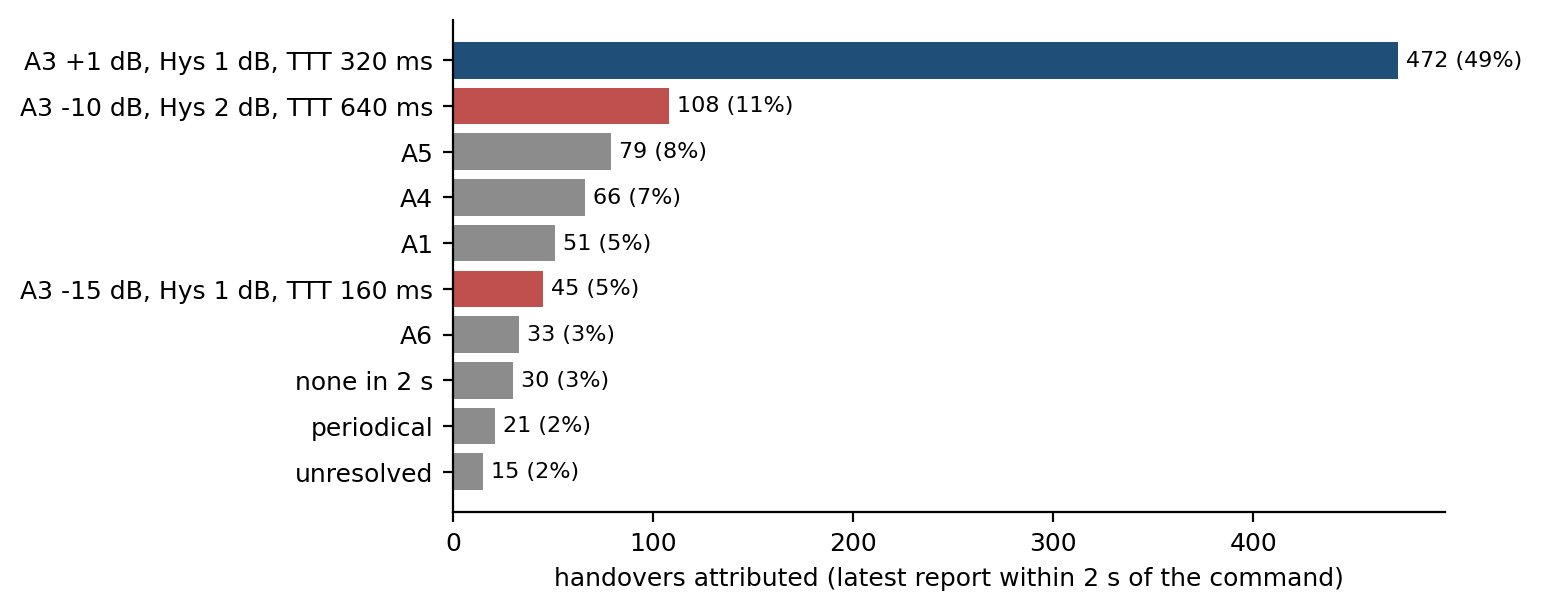
\includegraphics[width=0.85\linewidth]{figures/fig_c5_profiles.png}
\caption{Handovers attributed to each configuration profile, weighted by the handovers each actually produced. Almost three quarters of all A3-triggered handovers occur under positive offsets, dominated by the +1 dB profile.}
\label{fig:3_3}
\end{figure}


\section{The dataset}
\label{sec:3_6}


\begin{table}[htbp]
\centering
\caption{The four measurement campaigns after quality control. Handover command counts list total raw decoded commands followed parenthetically by quality-controlled commands falling inside retained 180~s blocks ($N = 938$, reconciled in Table~\ref{tab:3_reconciliation}).}
\label{tab:3_2}
\vspace{0.4em}
\singlespacing
\footnotesize
\resizebox{\linewidth}{!}{%
\begin{tabular}{l c c c c c c c c}
\toprule
\textbf{Campaign} & \textbf{Sessions} & \textbf{180 s blocks} & \textbf{Samples} & \textbf{Usable rows} & \textbf{Handover commands (Raw / Retained)} & \textbf{Re-establishments} & \textbf{Duration} & \textbf{Mean speed} \\
\midrule
1st Campaign (urban arterial) & 1 & 15 & 2,700 & 2,178 & 307 (290) & 113 & 45 min & 39.1 km/h \\
2nd Campaign (urban loop) & 1 & 8 & 1,440 & 1,131 & 176 (174) & 64 & 24 min & 25.0 km/h \\
3rd Campaign (dense urban) & 1 & 20 & 3,600 & 3,072 & 297 (297) & 159 & 60 min & 21.4 km/h \\
4th Campaign (highway) & 1 & 14 & 2,520 & 2,205 & 177 (177) & 5 & 42 min & 50.9 km/h \\
Pooled & 4 & 57 & 10,260 & 8,586 & 957 (938) & 341 & 2.9 h & --- \\
\bottomrule
\end{tabular}%
}
\end{table}


\begin{table}[htbp]
\centering
\caption{Ground-truth integrity. Every handover command in the decoded signalling is checked against the serving-cell sequence before and after it.}
\label{tab:3_3}
\vspace{0.4em}
\singlespacing
\footnotesize
\setlength{\tabcolsep}{2.5pt}
\begin{tabularx}{\linewidth}{p{2.9cm} *{6}{>{\centering\arraybackslash}X}}
\toprule
\textbf{Campaign} &
\shortstack{\textbf{Handover}\\\textbf{commands}} &
\shortstack{\textbf{Decoded}\\\textbf{Complete}} &
\shortstack{\textbf{Median log}\\\textbf{interval}} &
\shortstack{\textbf{Total}\\\textbf{re-est.}} &
\shortstack{\textbf{Re-est.}\\\textbf{$\le$\,5\,s of HO}} &
\shortstack{\textbf{Re-est.}\\\textbf{$\le$\,2\,s of HO}} \\
\midrule
1st Campaign (urban arterial) & 307 & 307 (100\%) & 1 ms & 113 & 19 & 30 \\
2nd Campaign (urban loop) & 176 & 176 (100\%) & 0 ms & 64 & 8 & 12 \\
3rd Campaign (dense urban) & 297 & 297 (100\%) & 1 ms & 159 & 5 & 13 \\
4th Campaign (highway) & 177 & 177 (100\%) & 1 ms & 5 & 4 & 0 \\
\midrule
Pooled & 957 & 957 (100\%) & 1 ms & 341 & 36 & 55 \\
\bottomrule
\end{tabularx}
\end{table}

The four campaigns cover 96 km of driving as recorded; the rows that survive to the modelling frame cover 78 km of that, and rates expressed per kilometre in Chapter 5 use the shorter figure, since that is the distance over which the model is scored. A handover command is issued on average once every 11 seconds, with a median inter-command gap of 3.7 seconds. Table~\ref{tab:3_3} also reconciles the two re-establishment counts, which do not match by design: Table~\ref{tab:3_2} counts every re-establishment in each session, while Table~\ref{tab:3_3} counts only those close to a handover command. The difference is the point --- most re-establishments in this corpus are not consequent on mobility at all, and the 286 that fall outside the two-second window after a command occur during ordinary connected-mode operation, predominantly at session start and after coverage gaps. Alongside the 957 commands, the signalling log records 341 RRC connection re-establishment procedures. Their causes matter and were decoded: 321 carry reconfigurationFailure, 17 otherFailure and 3 handoverFailure, and the median re-establishment occurs 8 seconds after the previous handover command. These are predominantly failures to apply a reconfiguration rather than radio link failures during mobility, and they are treated as a competing event in Section~\ref{sec:5_8} rather than as a motivating statistic.


\begin{figure}[htbp]
\centering

\includegraphics[width=0.90\linewidth]{figures/fig05_dataset.png}
\caption{Composition of the pooled dataset across the four campaigns. In the event panel, counts reflect the $N = 938$ handover commands falling within retained quality-controlled blocks (290, 174, 297, and 177 respectively), which feed the feature pipeline, drawn from the 957 total decoded commands in Table~\ref{tab:3_2}.}
\label{fig:3_4}
\end{figure}

A rate of one re-establishment per three handover commands invites the question whether the commands themselves succeeded, since a label that means only a command was issued would make every event-level figure in this thesis uncertain. To ensure ground-truth integrity, the event set was filtered to commands with a confirmed completion: each handover command was extracted as an RRCConnectionReconfiguration message containing mobilityControlInfo, matched to its corresponding RRCConnectionReconfigurationComplete message via RRC transaction identifier and carrier context. Across the four campaigns, all 957 retained commands in the event set carry a decoded RRCConnectionReconfigurationComplete (100\%); thus, the model predicts commands that resulted in completed execution rather than abandoned attempts. In Table~\ref{tab:3_3}, the median logging timestamp interval between the command and completion decode is 0--1 ms (reflecting instantaneous logging of back-to-back signaling PDUs rather than user-plane interruption duration, which 3GPP TS 36.331 defines across lower-layer synchronization). Only 36 commands are followed by a re-establishment within five seconds, and only 55 of the 341 re-establishments fall within two seconds after a command. The re-establishments are therefore concurrent with the measurement campaign rather than consequent on the handovers it records, which is what the cause breakdown already implied and what this check establishes. Table~\ref{tab:3_3} reports the completion rate and timing per campaign. Figure~\ref{fig:3_4} shows the distribution of samples and events across the campaigns.

The dataset is small by machine-learning standards and ordinary by drive-test standards. Four campaigns give four independent units; the 57 blocks into which they are cut are not independent, and Section~\ref{sec:5_3} measures the difference. Four units is enough to hold one out at a time and to see whether a result survives, and too few for any paired test over units to reach a small p-value: with four paired observations the smallest attainable two-sided sign-test p-value is 0.125, and this thesis reports effect sizes and per-campaign spreads rather than significance claims.

The sampling rate and preprocessing rules jointly determine the eligible-prediction-window ceiling. On an uninterrupted integer-second grid, every interior event has a sample point in the preceding second (for example, an event at 12.7 s has a grid instant at 12.0 s). However, under the evaluation policy adopted here, prediction rows are blanked for two seconds following each handover to suppress post-transition transients, and boundary rows lacking rolling history are excluded. Consequently, closely spaced handovers inside bursts and boundary events lack an eligible prediction row. The fraction of handover commands that have at least one eligible prediction row inside the one-second window before them is 64.2\% (leaving 35.8\% unresolvable in the pooled sequence, predominantly due to the 2 s blanking window during bursts; in chunk-split calibration folds, additional boundary cuts raise the unresolvable share to 36.4\%). Event-level detection figures are therefore reported against this eligible-window ceiling rather than against 100 \%.

The configuration in Table~\ref{tab:3_1} is one operator's configuration, and the independent collection used in Section~\ref{sec:5_7} is on the same operator, same city and same instrument, so it tests collection and route rather than network.

